\section{Database Setup}

In this paragraph we illustrate a basic postgres setup, replace the $<>$ fields with your information.\\

\noindent Install the postgres package
\begin{lstlisting}[language=bash]
$ sudo apt-get install postgresql postgresql-contrib
\end{lstlisting}
\bigskip
Create a new postgres user
\begin{lstlisting}[language=bash]
$ sudo -u postgres createuser <username>
\end{lstlisting}
\bigskip
Create a new database
\begin{lstlisting}[language=bash]
$ sudo -u postgres createdb <dbname>
\end{lstlisting}
\bigskip
Open postgres console
\begin{lstlisting}[language=bash]
$ sudo -u postgres psql
\end{lstlisting}
\bigskip
Assign a password to the user
\begin{lstlisting}[language=bash]
$ (postgres) alter user <username> with encrypted password <password>;
\end{lstlisting}
\bigskip
Grant privileges to the user over the database
\begin{lstlisting}[language=bash]
$ (postgres) grant all privileges on database <dbname> to <username>;
\end{lstlisting}
\bigskip
\noindent
if you plan to install the DBMS on a different machine from that of the application you may want to enable port forwarding and change postgres setup to allow external requests.

\section{Mail Account}

You may want to create a new email account which will be used to send email on behalf of the application, in our configuration we used Gmail but any mail provider should be fine.

\section{External Services Setup}

In this paragraph we illustrate the necessary setup for the external services API used.

\subsection{Google API}
In order to get the Google API key follow the instructions in the following link
\begin{center}
	\hyperref{https://developers.google.com/maps/documentation/directions/get-api-key}{}{}{https://developers.google.com/maps/documentation/directions/get-api-key}
\end{center} 

\subsection{MapBox API}
In order to get the MapBox API key sign up using the following link
\begin{center}
	\hyperref{https://www.mapbox.com}{}{}{https://www.mapbox.com}
\end{center}
Once logged in, go to account$\rightarrow$dashboard and create a new token selecting the scopes "DATASETS:READ", "DATASETS:LIST" and "DATASETS:WRITE".

\subsection{Uber API}
In order to get the Uber API key sign up using the following link
\begin{center}
	\hyperref{https://developer.uber.com}{}{}{https://developer.uber.com}
\end{center}
Once logged, create a new App. From the dashboard is possible to get the \textit{Server Token}.\\
Once the iOS application is created, the following changes have to be applied:
\begin{itemize}
	\item In the Dashboard Auth page, edit the \textit{redirect URI} field with
	\begin{center}
		\textit{$<$APPLICATION BUNDLE ID$>$://oauth/consumer}
	\end{center} 
	\item In the Dashboard$\rightarrow$Settings$\rightarrow$Security, edit the \textit{App Signatures} with
	\begin{center}
		\textit{$<$APPLICATION BUNDLE ID$>$}
	\end{center}
\end{itemize}
In order to use Uber with more accounts, in the Dashboard$\rightarrow$Developers settings the Uber accounts must be added.

\subsection{Usage of the keys}
Once all the keys are retrieved, open the file \textit{ApiKeys.php} (\textit{app/Http/Helper/ApiKeys.php}) and edit the variable value:
\begin{lstlisting}[language=bash]
	$googleKey = <YOUR GOOGLE API KEY>
\end{lstlisting}

\begin{lstlisting}[language=bash]
	$mapboxKey = <YOUR MAPBOX API KEY>
\end{lstlisting}

\begin{lstlisting}[language=bash]
	$uberServerToken = <YOUR UBER SERVER TOKEN>
\end{lstlisting}
	
\begin{lstlisting}[language=bash]
	$uberClientToken = <YOUR UBER CLIENT TOKEN>
\end{lstlisting}
N.B. This key is used only used in order to test the application. This key is available only after the authentication in the Uber application. The Authentication protocol is omitted.

\section{Application Back-end Setup}

In this paragraph we illustrate how to install the dependencies and initialize the application.\\

\subsection{Instructions}

\noindent Install Laravel dependencies
\begin{lstlisting}[language=bash]
$ sudo apt-get install php
\end{lstlisting}
\begin{lstlisting}[language=bash]
$ sudo apt-get install openssl
\end{lstlisting}
\begin{lstlisting}[language=bash]
$ sudo apt-get install php7.1-pgsql
\end{lstlisting}
\begin{lstlisting}[language=bash]
$ sudo apt-get install php7.1-mbstring
\end{lstlisting}
\begin{lstlisting}[language=bash]
$ sudo apt-get install php7.1-xml
\end{lstlisting}
\bigskip
Install other dependencies
\begin{lstlisting}[language=bash]
$ sudo apt-get install curl
\end{lstlisting}
\begin{lstlisting}[language=bash]
$ sudo apt-get install php7.1-curl
\end{lstlisting}
Install PHP dependency manager
\begin{lstlisting}[language=bash]
$ sudo apt install composer
\end{lstlisting}
Install Python package manager
\begin{lstlisting}[language=bash]
$ sudo apt install python3-pip
\end{lstlisting}
Install python package for CSP
\begin{lstlisting}[language=bash]
$ pip3 install python-constraint
\end{lstlisting}

\bigskip
\noindent Decompress the zip file containing the application files.\\
Configure your '.env' file in the root folder of the project filling the $<>$ fields with your information, the other fields may be left empy or with the default values.
\bigskip
\begin{lstlisting}
APP_NAME=Travlendar
APP_ENV=local
APP_KEY=
APP_DEBUG=true
APP_LOG_LEVEL=debug
APP_URL=http://localhost

DB_CONNECTION=<dbms identifier or pgsql for postgres>
DB_HOST=<dbaddress or 127.0.0.1 if db is local>
DB_PORT=<dbport or 5432 as default>
DB_DATABASE=<dbname>
DB_USERNAME=<username>
DB_PASSWORD=<password>

BROADCAST_DRIVER=log
CACHE_DRIVER=file
SESSION_DRIVER=file
SESSION_LIFETIME=120
QUEUE_DRIVER=database

REDIS_HOST=127.0.0.1
REDIS_PASSWORD=null
REDIS_PORT=6379

MAIL_DRIVER=smtp
MAIL_HOST=<mail host or smtp.gmail.com for gmail>
MAIL_PORT=587
MAIL_USERNAME=<mailaccount>
MAIL_PASSWORD=<mailpassword>
MAIL_ENCRYPTION=tls
MAIL_FROM_ADDRESS=<mailaddress>
MAIL_FROM_NAME=Travlendar+

PUSHER_APP_ID=
PUSHER_APP_KEY=
PUSHER_APP_SECRET=
\end{lstlisting}
\bigskip
\noindent
From the root folder of the project.

\bigskip
\noindent
Generate an application key
\begin{lstlisting}[language=bash]
$ php artisan key:generate
\end{lstlisting}
Migrate the tables to the database
\begin{lstlisting}[language=bash]
$ php artisan migrate --seed
\end{lstlisting}
Generate oauth keys
\begin{lstlisting}[language=bash]
$ php artisan passport:install
\end{lstlisting}
\bigskip
Remove from the 'composer.json' file
\begin{lstlisting}[language=bash]
"phpunit/phpunit": "~6.0"
\end{lstlisting}
Run
\begin{lstlisting}[language=bash]
$ composer update
\end{lstlisting}
Add the previously deleted line and rerun the update.\\
(This may seem unnecessary but it fixes a missing symlink caused by migrating the project and allows to run the test suite).\\

\noindent Start Laravel Development Server
\begin{lstlisting}[language=bash]
$ php artisan serve --host=<host_addr> --port=<port>
\end{lstlisting}

\noindent Run the tests
\begin{lstlisting}[language=bash]
$ vendor/bin/phpunit
\end{lstlisting}

\section{Client Application Setup}
In this section, all the relevant information to build the iOS application are provided as clearly as possible.

\subsection{Requirements}

\begin{itemize}
	\item OSX with Xcode 9.x
	\item Apple ID
	\item Internet connection
	\item (Optional) iPhone with iOS 10+
\end{itemize} 

\subsection{How to build}

In order to build the application, you need to open with Xcode the file \textit{Trav.xcworkspace} inside the iOS/Trav folder.

The indexing phase may take up to one or two minutes. Then, choose a simulator device at the top left corner of the Xcode and press the play button to build. Alternatively, you can connect your own iPhone and run the app on it directly.

\begin{figure}[H]
	\centering
	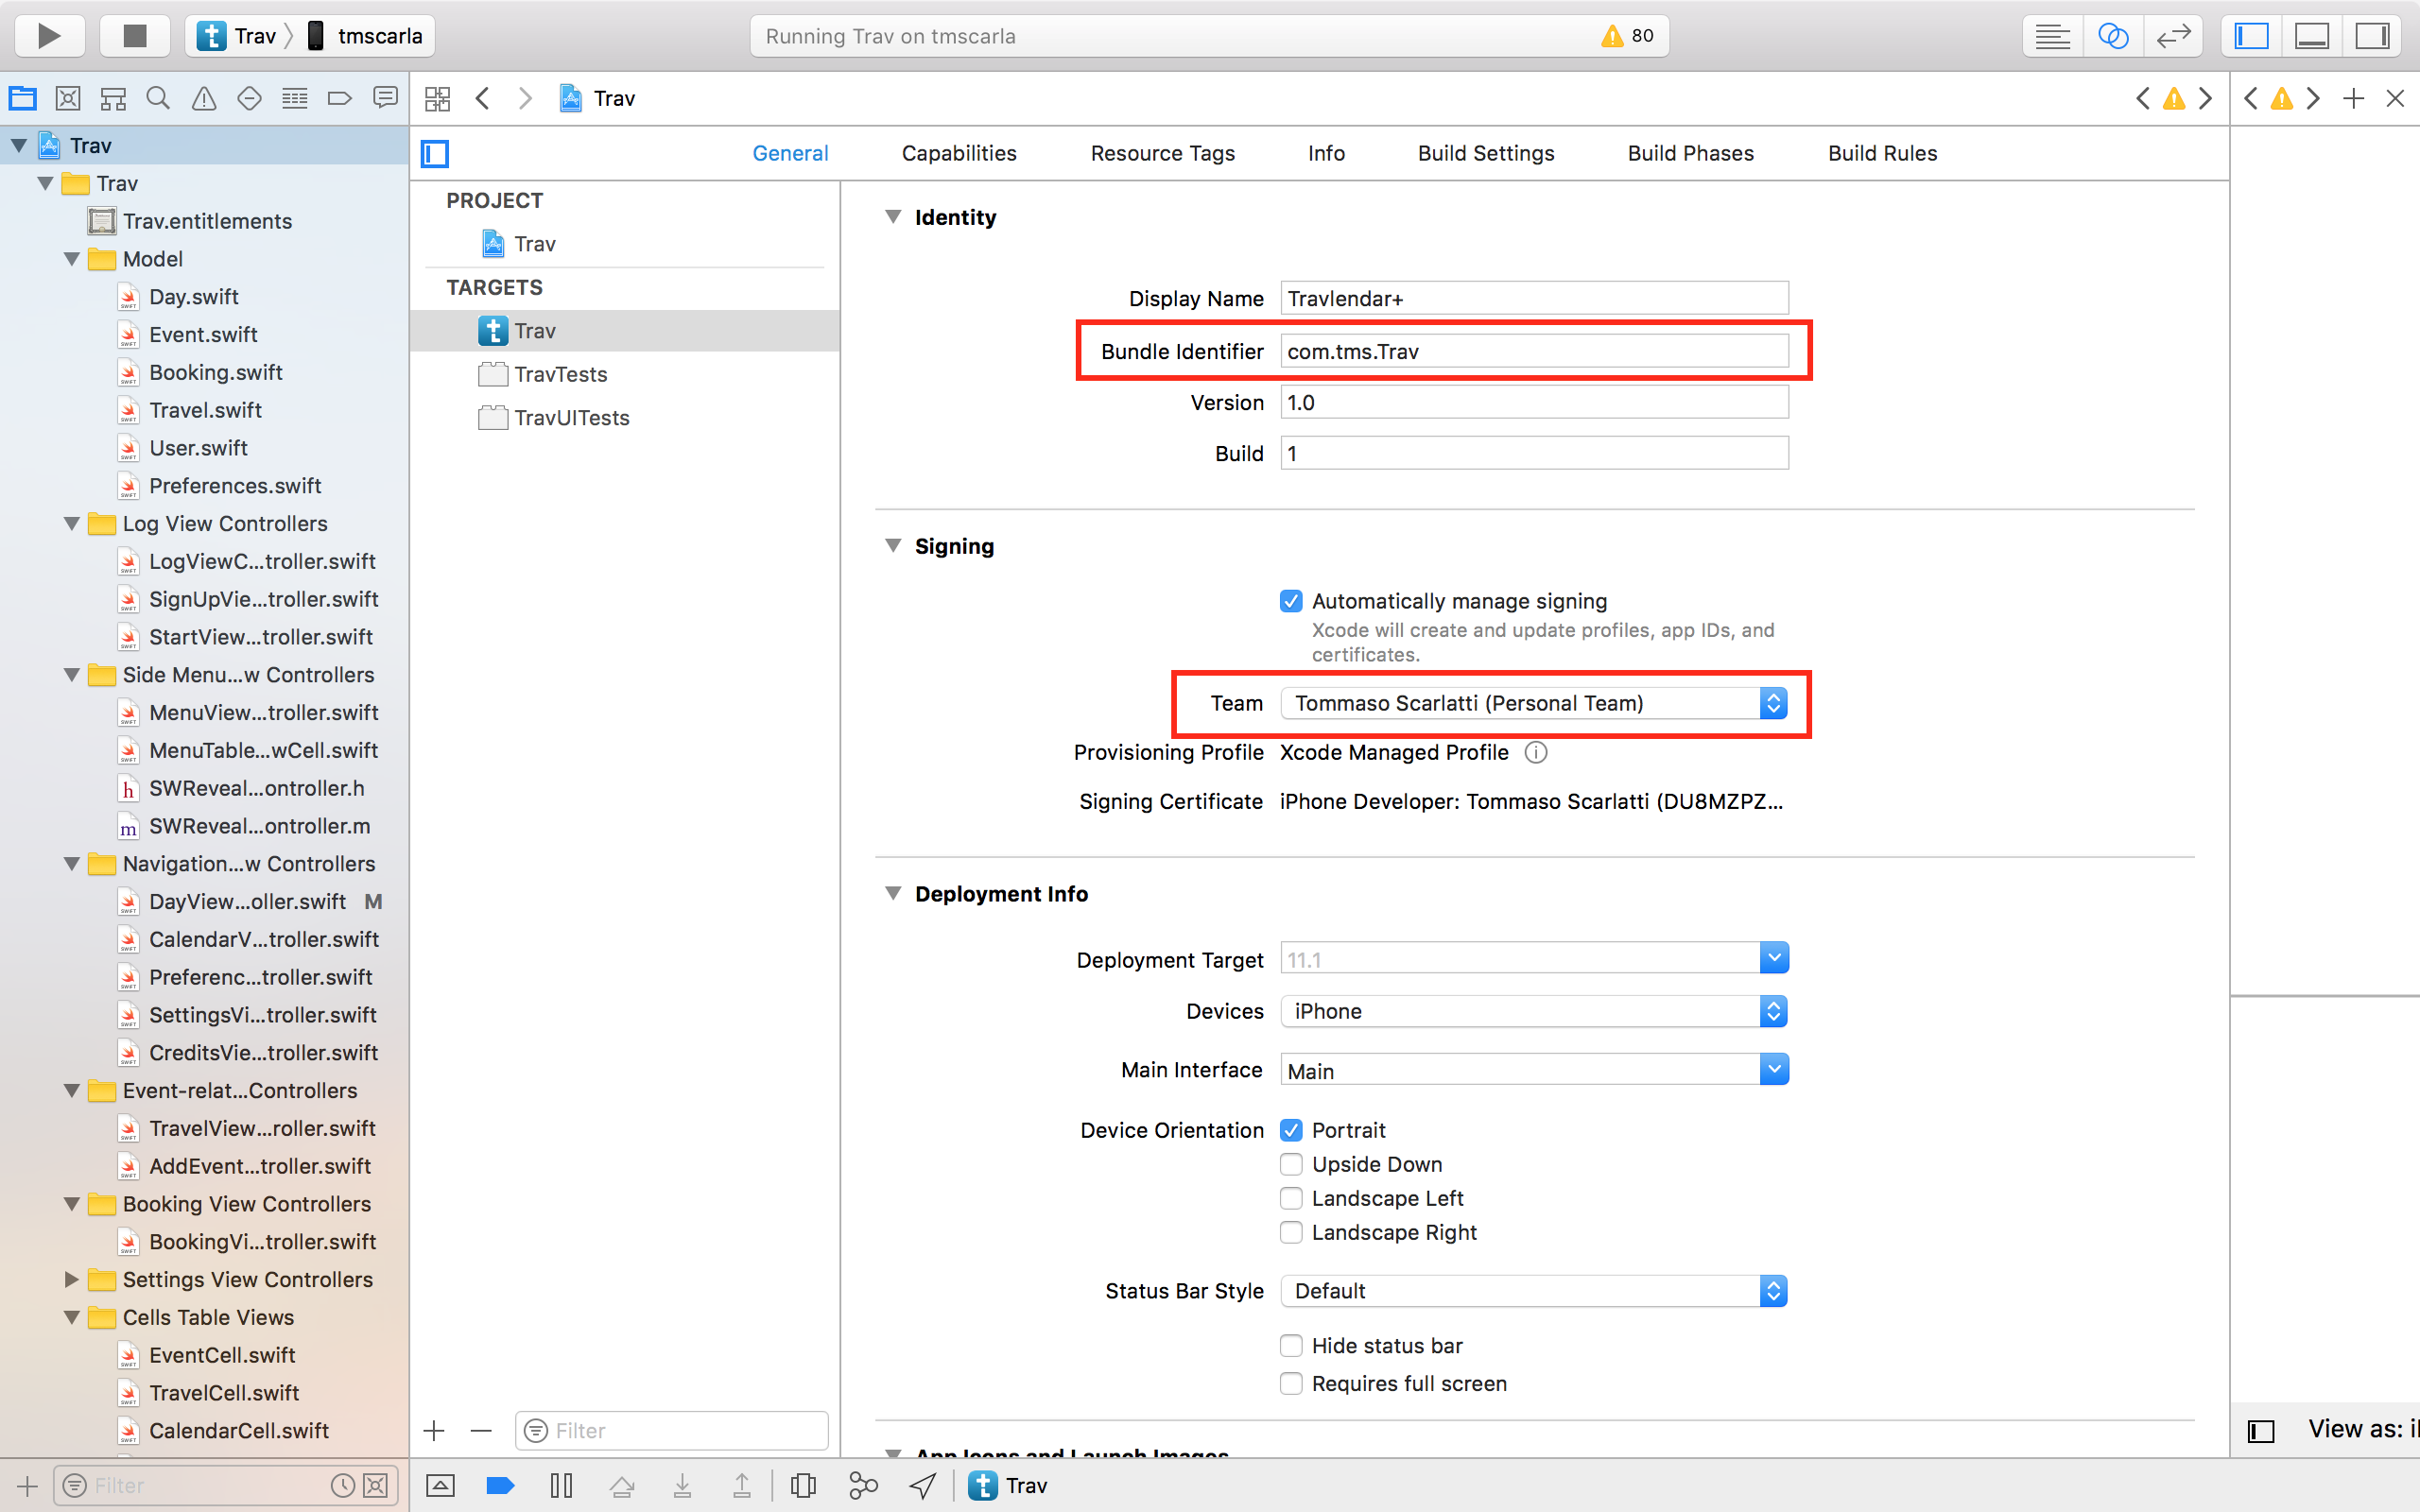
\includegraphics[scale=0.30]{bundle.png}
	\caption{General options}
\end{figure}

You have to change the team name with your personal Apple ID (or a team name, if you have one) and consequentely the Bundle Identifier, as shown in the image above.

\subsubsection*{Info.plist}
Inside the project folder you can find a file called \textit{Info.plist}, which is a structured text file that contains essential configuration information for a bundled executable.
It is basically a dictionary with a [key : value] mapping.

At the bottom of the list you can find to keys: \textit{Server Name} and \textit{Travlendar Client Secret} that can be both easily replaced in case you want to set up the back end on a different server.

Here you can also find the keys related to the Uber iOS sdk setup if you want to change them in order to make your account elegible to perform rides requests.

\begin{figure}[H]
	\centering
	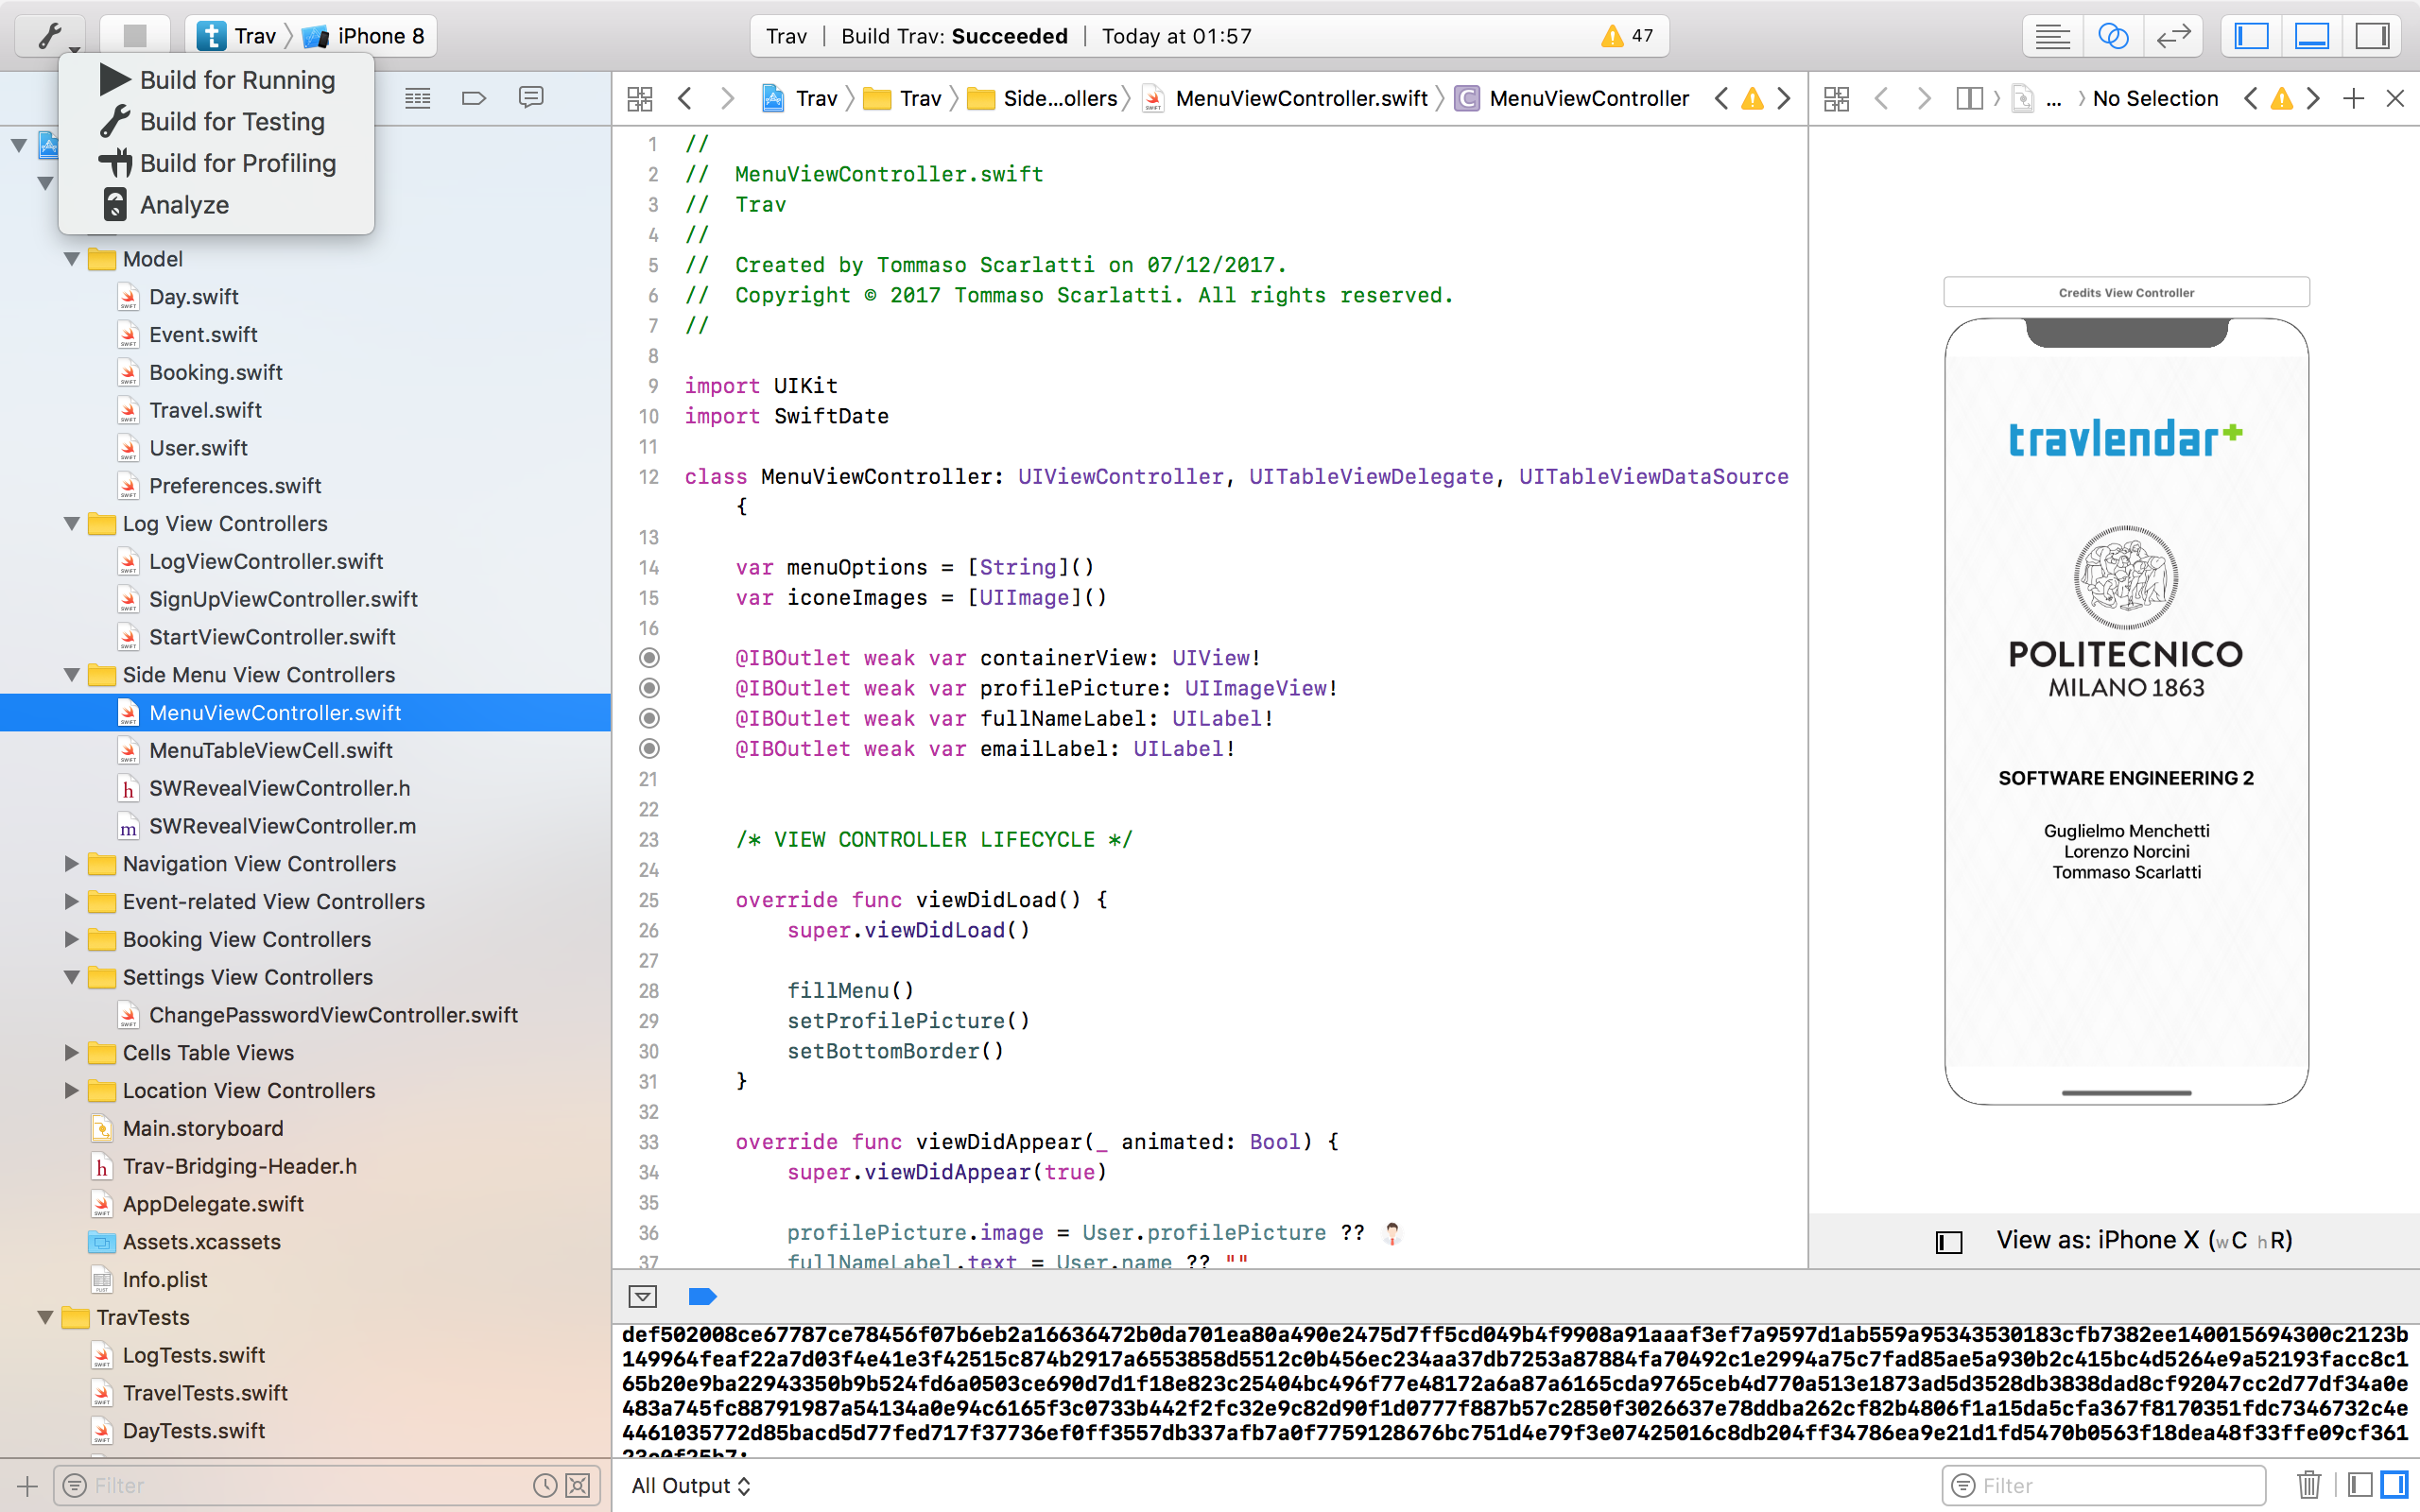
\includegraphics[scale=0.3]{xcode_screenshot.png}
	\caption{Build options}
\end{figure}

\subsection{How to test}

If you want to perform the integration tests for the HTTP request to the server you can hold the play button, as in the figure above, and choose the "Build for Testing" option.
Doing like this will build all the tests located in the "TravTest" folder.

If you want to perform a single test, you can swap the left view form the current \textit{Project navigator} to the \textit{Test navigator}.

\begin{figure}[H]
	\centering
	
\includegraphics[scale=0.8]{xcode_navbar.png}
	\caption{Project navigator and Test navigator}
\end{figure}


\subsection{Known issues}

\begin{itemize}
	\item \textbf{Auto-layout warnings}: there are plenty of warnings due to UI constraints.
	\item \textbf{UI issues}: the application was tested on the iPhone 8 simulator and on a physical iPhone 7. Due to constraints warnings, the view may not perform as expected.
	\item \textbf{Uber requests}: due to limitations imposed by Uber, you need to setup your personal Uber developer account in order to make Uber rides requests, as explained in section 4.3.
\end{itemize}